\documentclass[DIV=14]{scrartcl}
\usepackage[utf8]{inputenc}
\usepackage[T1]{fontenc}  % needed for the correct underscores in \texttt
\usepackage{graphicx}
\usepackage{amsmath}
\usepackage{physics}

\usepackage{siunitx}
\DeclareSIUnit{\LSB}{LSB}

\usepackage{hyperref}
\hypersetup{pdfborder = 0 0 0}  % links without decoration

\usepackage{censor} % just for the sample report, no use in a real report

\titlehead{
    Laboratory for Electrical Instrumentation and Embedded Systems \\
    IMTEK -- Department of Microsystems Engineering \\
    University of Freiburg \vspace{0.5cm} \\
    Sensors Lab Course \\
    Winter term 2022/23 \vspace{1.5cm}}

\title{Lab Report M1}
\subtitle{Acceleration and Pressure Sensors}
\author{Rafael Andrioli Bauer (5163344)}

\begin{document}

    \maketitle

    \thispagestyle{empty}

    \vfill
    \begin{center}
        
\includegraphics{ufcd-logo-e1-a4-color.pdf} \vspace{1cm} \\
    \end{center}
    \vfill

% Comment out the entire 'flushleft' block if you did the experiments alone
%\begin{flushleft}
%Data generated in a team together with
%\begin{itemize}
%    \item Robert Hooke (2718281)
%    \item Edmond Halley (1414213)
%\end{itemize}
%\end{flushleft}

    \clearpage


    \section{Introduction}
    Dynamic systems are present in our day-to-day and elevators is one of them.
    They play a very important role in the modern world, making vertical transportation easier and helping people
    to reach their destinations faster.
    In this module, the accelerometer and barometric sensors of the Nicla Sense ME Board were investigated in an elevator.
    The elevator height is measured using the pressure sensor and by integrating twice the acceleration.
    A discussion of which approach is better is done.
    Before, the accelerometer and barometric sensors are characterized for offset and noise.

    \section{Theory}
    By definition, acceleration $a$ is the rate of change of the velocity $v$ in time and the velocity is the rate
    of change of the position $s$.
    It is expressed as
    \begin{equation}
        a = \dv{v}{t} = \dv[2]{s}{t}.
        \label{eq:accelerationDefinition}
    \end{equation}

    Trivially when integrating the acceleration once we can compute the speed at a time point $t$, and integrating
    it twice we can compute the position.
    Intuitively when having the accelerometer axis perpendicular to the floor, one can measure the change in height.

    Another way to perform the same measurement is to use a barometric sensor.
    There is a relation between the pressure and the height above sea level~\cite{labManual}
    \begin{equation}
        p = p_0 \exp(-\frac{gMh}{RT}),
        \label{eq:pressure}
    \end{equation}
    where $p$ is the pressure, $p_0$ is the reference pressure and $h$ is the height.
    The equation counts with some constants such as gravity acceleration $g = 9.81\frac{\mathrm{m}}{\mathrm{s}^2}$,
    the molar mass of air $M = 0.02896\frac{\mathrm{kg}}{\mathrm{mol}}$ and the universal gas constant
    $R = 8.314\frac{\mathrm{J}}{\mathrm{mol}\mathrm{K}}$

    When isolating $h$
    \begin{equation}
        h = (\ln(p_0) - \ln(p))\frac{RT}{gM},
        \label{eq:pressureHeight}
    \end{equation}
    one can derive the height change and cancel out the reference pressure $p_0$
    \begin{equation}
        \Delta h = h_2 - h_1 = \ln(\frac{p_1}{p_2})\frac{RT}{gM}.
        \label{eq:relativePressureHeight}
    \end{equation}

    The pressure must be in $\si{\hecto\pascal}$ and the height will be in meters.

    \subsection{Barometric Sensor}\label{subsec:barometric-sensor}
    Arduino Nicla has the barometric sensor BMP390, from Bosch Sensortech.
    Such sensor is based in the pressure-gradient force ($PFG$) which is the force that results when there is difference in
    pressure across a surface.
    It is defined as~\cite{Hautala}
    \begin{equation}
        PFG = -\frac{1}{\rho}\nabla{P} = -\frac{1}{\rho}(\pdv{P}{x},\pdv{P}{y},\pdv{P}{z})
        \label{eq:pressureGradientForce},
    \end{equation}
    where $\rho$ is the fluid density and $P$ the pressure.

    The sensor is constructed in a way that it contains a micro-fabricated membrane that deflects due to the $PSG$.
    The deflection changes piezoresistive elements connected to a circuit resulting in a voltage change.
    Figure~X illustrates the construction of such sensor.

    TODO: Figure here
%    \begin{figure}[h]
%        \centering
%        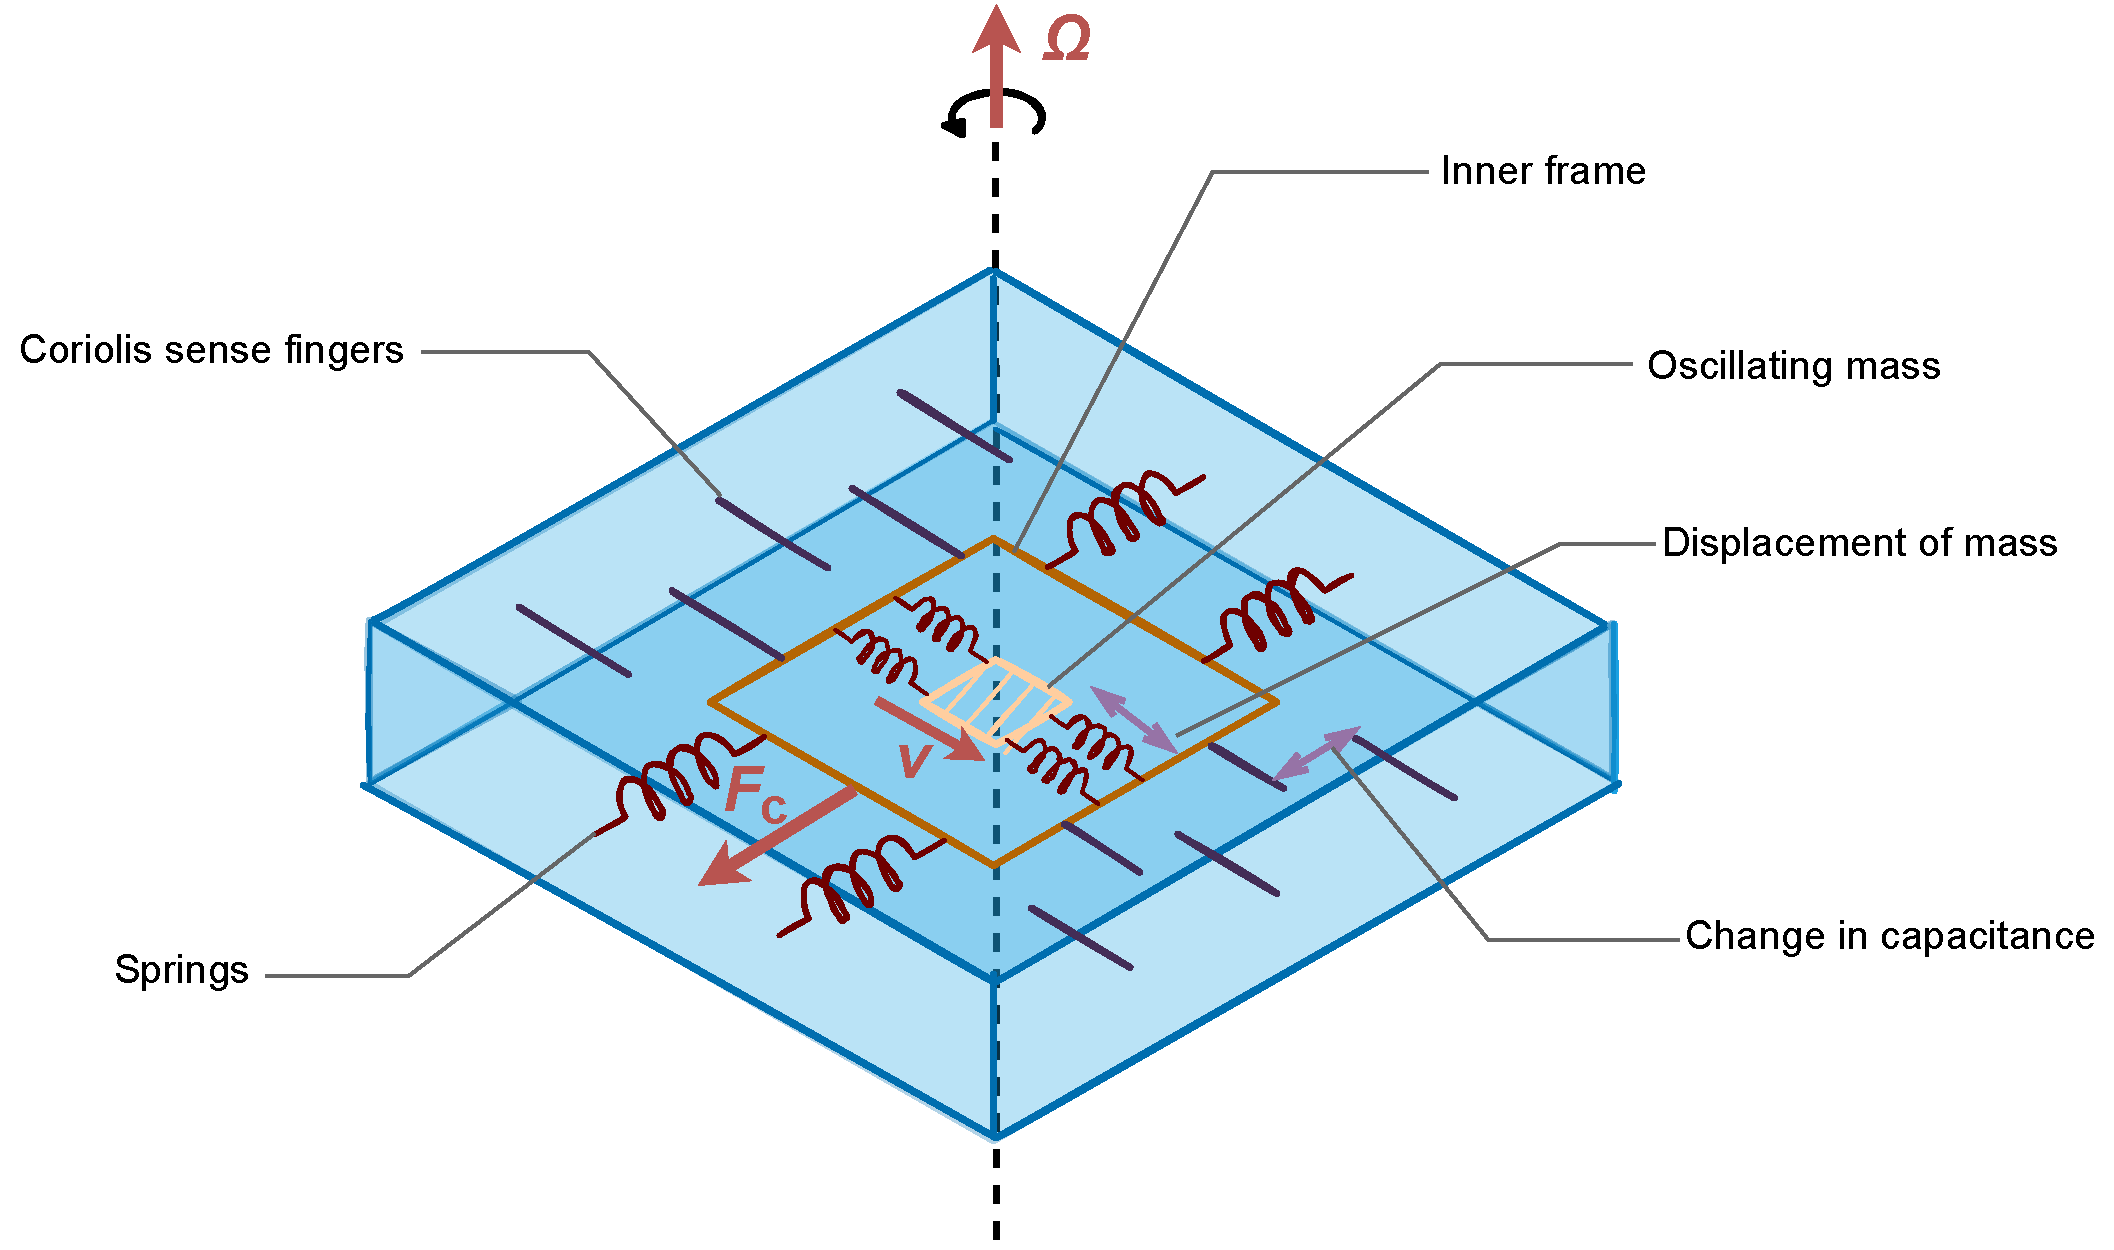
\includegraphics[width=.8\textwidth]{figures/gyroscope.drawio.pdf}
%        \caption{Principle of a micro-fabricated pressure sensor to measure the barometric pressure
%                 of the air. (author's own work).}
%        \label{fig:barometer}
%    \end{figure}

%    The BMP390 is an absolute pressure sensor where which one of the cavities is sealed by the membrane with a reference
%    pressure and the other can be accessed from the outside.
%    The change in pressure

    \subsection{Acceleration Sensor}
    Accelerometers, as the name itself already says, measures acceleration.
    It does so based on Newton's second law
    \begin{equation}
        F = ma
        \label{eq:newtonsLaw},
    \end{equation}
    by observing the force acting on a mass~\cite{labManual} (seismic mass) which is suspended by springs.
    The position of the mass is read by comb-like structures, and the mass movement results in change in capacity
    between neighboring fingers~\cite{labManual}.

    The typical setup of Micro electromechanical system (MEMS) accelerometers is shown in Figure~\ref{fig:accelerometer}
    \begin{figure}[h]
        \centering
        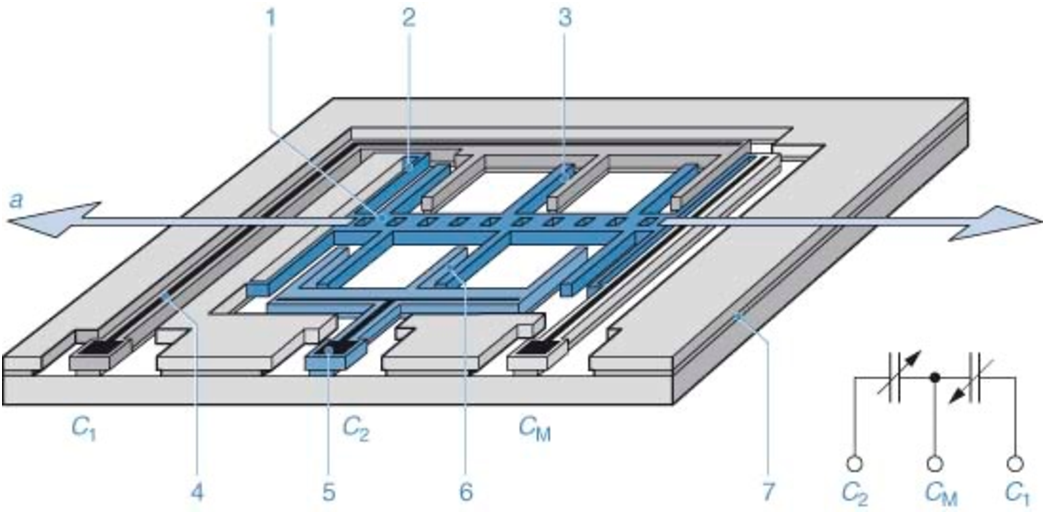
\includegraphics[width=.6\textwidth]{figures/accelerometer}
        \caption{Principle of a microfabricated, capacitive accelerometer to sense the in-plane acceleration (Bosch Gmbh).}
        \label{fig:accelerometer}
    \end{figure}

    \clearpage


    \section{Methods}
    All measurements used the BHI260AP of an Arduino Nicla Sense Board ME connected via USB to a battery-powered
    notebook acting both as a power supply for the board and data logger.
    The board was programmed using the Arduino IDE 2.0.2 with the \texttt{Arduino\_BHY2} library version 1.0.5 (Bosch Sensortec).
    A small MATLAB application called \textit{SampleNicla} was developed to log the data.
    MATLAB was also used to process the data.
    The source code is available in \href{https://github.com/RafasLectures/sensorslab/blob/main/SampleNicla.mlapp}{GitHub}
    (\texttt{https://github.com/RafasLectures/sensorslab/})

    In a \SI{10}{\hertz} sampling rate (every \SI{100}{\milli\second}), the Arduino program reads the acceleration
    virtual sensors \texttt{SENSOR\_ID\_ACC\_PASS} and the barometric sensor
    \texttt{SENSOR\_ID\_BARO} from the BHI260AP.
    The sensitivity of the acceleration sensor was \SI{1670.13}{\frac{\LSB}{\mathrm{m/s^2}}} (2$g$ range) and the
    barometer had a relative accuracy of $\pm$\SI{3}{\pascal} \cite{BHI260}.

    The data acquisition for Task~1 and 2 were performed at the same time.
    The sensor was placed in a flat surface with its $z$-axis pointing upwards (Figure~\ref{fig:setup}).

    For Task~3, the elevator ride was performed in a 5 stories residential building in Freiburg.
    The sensor was placed in the middle of the cabin with its $z$-axis pointing upwards (Figure~\ref{fig:setup}).
    Two rides were performed, one upward and another downwards.
    The first ride started at the lowermost landing up to the 5\textsuperscript{th} floor and the other was the
    other way around.
    The sampling never stopped between the two rides, and before each ride there was a period where the elevator
    stayed in the landing with doors open.

    The measurements of Tasks~1, 2 and 3 were recorded at approximately \SI{20}{\celsius} (indoor).

    \vspace{3em}

    \begin{figure}[h]
        \centering
        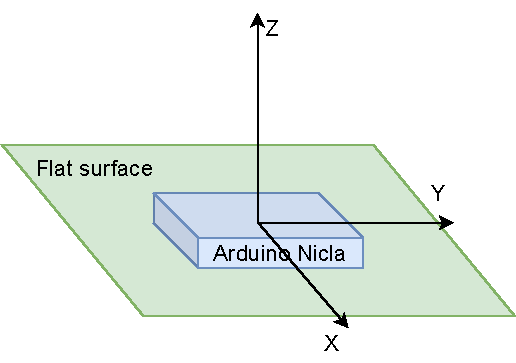
\includegraphics[width=.6\textwidth]{figures/Setup1and2}
        \caption{Setup of Task~1, 2 and 3: the sensor was placed in a flat surface with its $z$-axis pointing upwards
            (author's own work).}
        \label{fig:setup}
    \end{figure}

    \clearpage


    \section{Results and Discussion}

    \subsection*{Task 1}
    The first task is intended to verify the performance of the pressure sensor.
    The noise level and the offset are evaluated in this task.
    The Nicla Sense ME Board was placed flat on a steady table and the pressure was recorded.
    The obtained values are in already in \si{\hecto\pascal}.
    No drift is visible.
    An offset of 981.81 \si{\hecto\pascal} is seen.
    It is expected since the pressure at sea level is 1013.25 \si{\hecto\pascal} and we are above sea level,
    so the offset should be slightly below the pressure at sea level.
    Figure~\ref{fig:plotPressure} provides an overview on the 1,000 pressure samples.

    \begin{figure}[h]
        \centering
        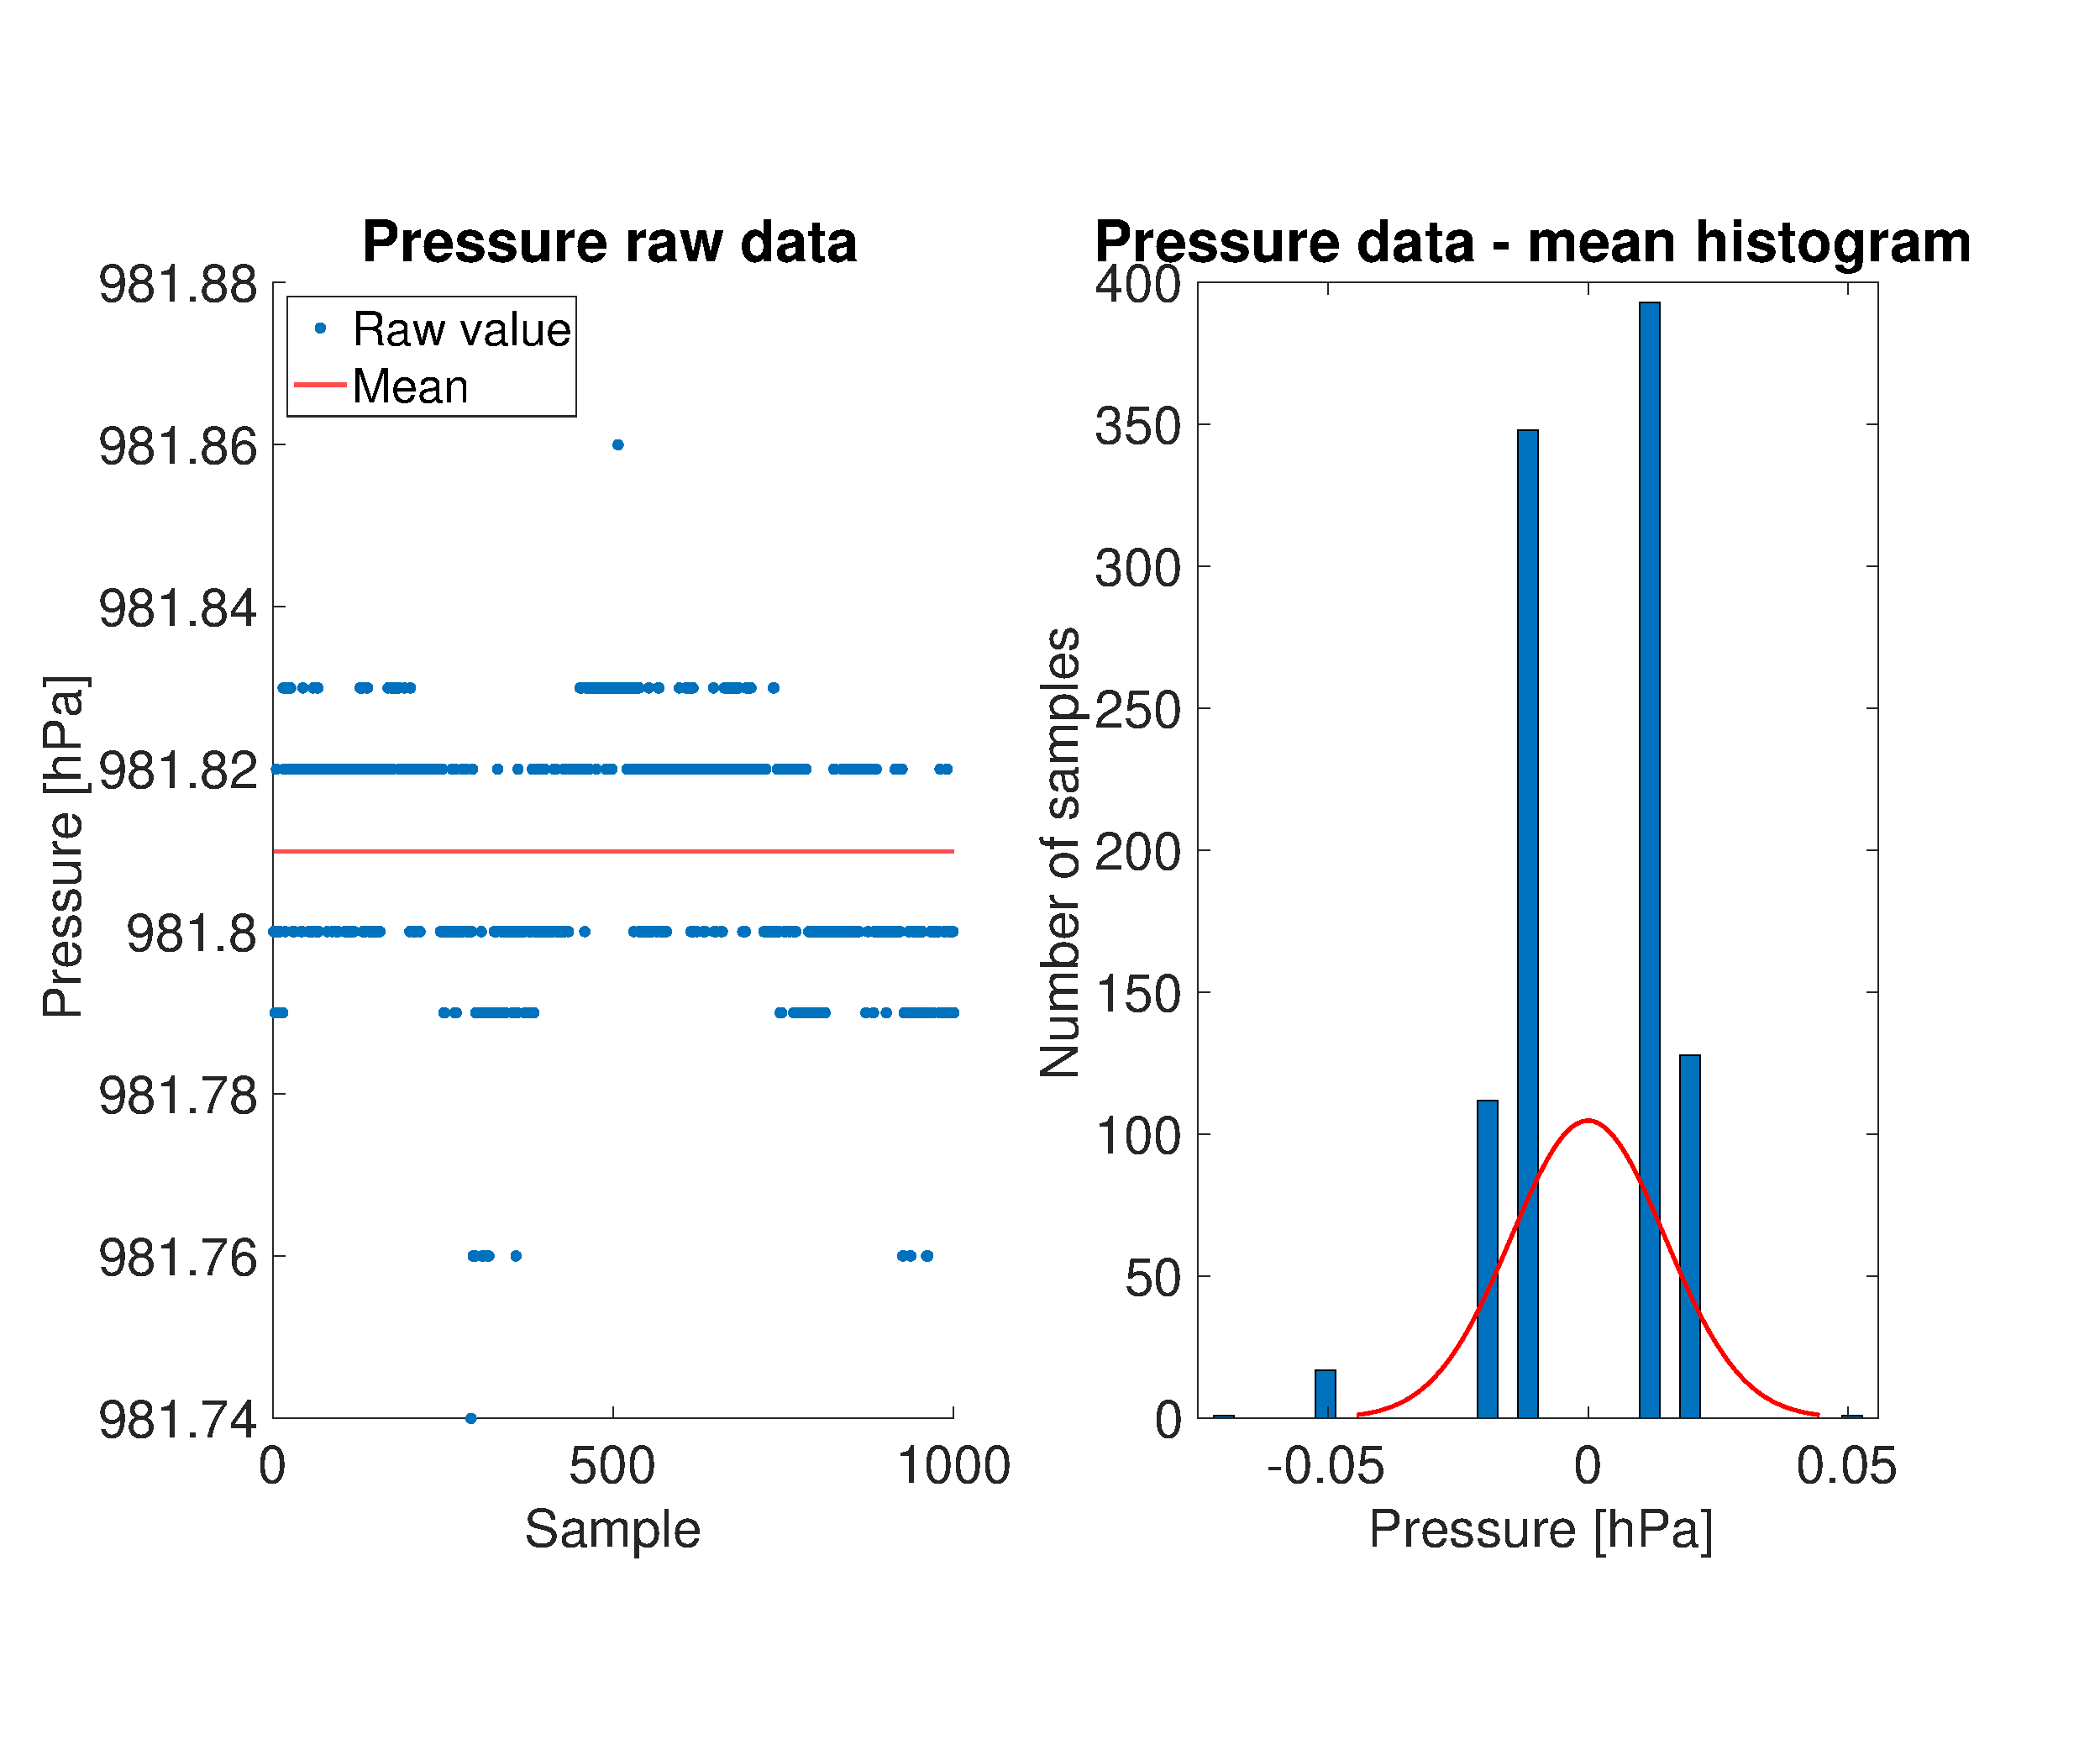
\includegraphics[width=.6\textwidth]{plots/plotPressure}
        \caption{Pressure readings at rest. The measurement rate is \SI{10}{\hertz}.}
        \label{fig:plotPressure}
    \end{figure}

    The mean value $\bar{p}$ (offset) is 9.81 \si{\hecto\pascal} and the standard deviation $\sigma_p$ is 0.014 \si{\hecto\pascal}
    The histogram shows that the values follow a normal distribution.
    The values are according to the datasheet, which specifies an accuracy of $\pm3 \si{\pascal}$ and
    the standard deviation is within that range.

    \clearpage


    \subsection*{Task 2}
    The second task is intended to verify the performance of the accelerometer.
    The noise level and the offset are evaluated in this task.
    The Nicla Sense ME Board was placed flat on a steady table and the acceleration on the $x$, $y$ and $z$-axis were recorded.
    No drift is visible and an offset of 9.99 \si{\frac{\meter}{\second^2}} is seen only in the $z$-axis.
    The offset is expected since it is the same axis as gravity.
    The value is a little above than 9.81\si{\frac{\meter}{\second^2}} and the reason can be due to calibration of
    the accelerometer.

    Figure~\ref{fig:accelerationHist} shows the raw data together with the histogram of the raw data subtracted by the mean.

    \begin{figure}[h]

        \centering
        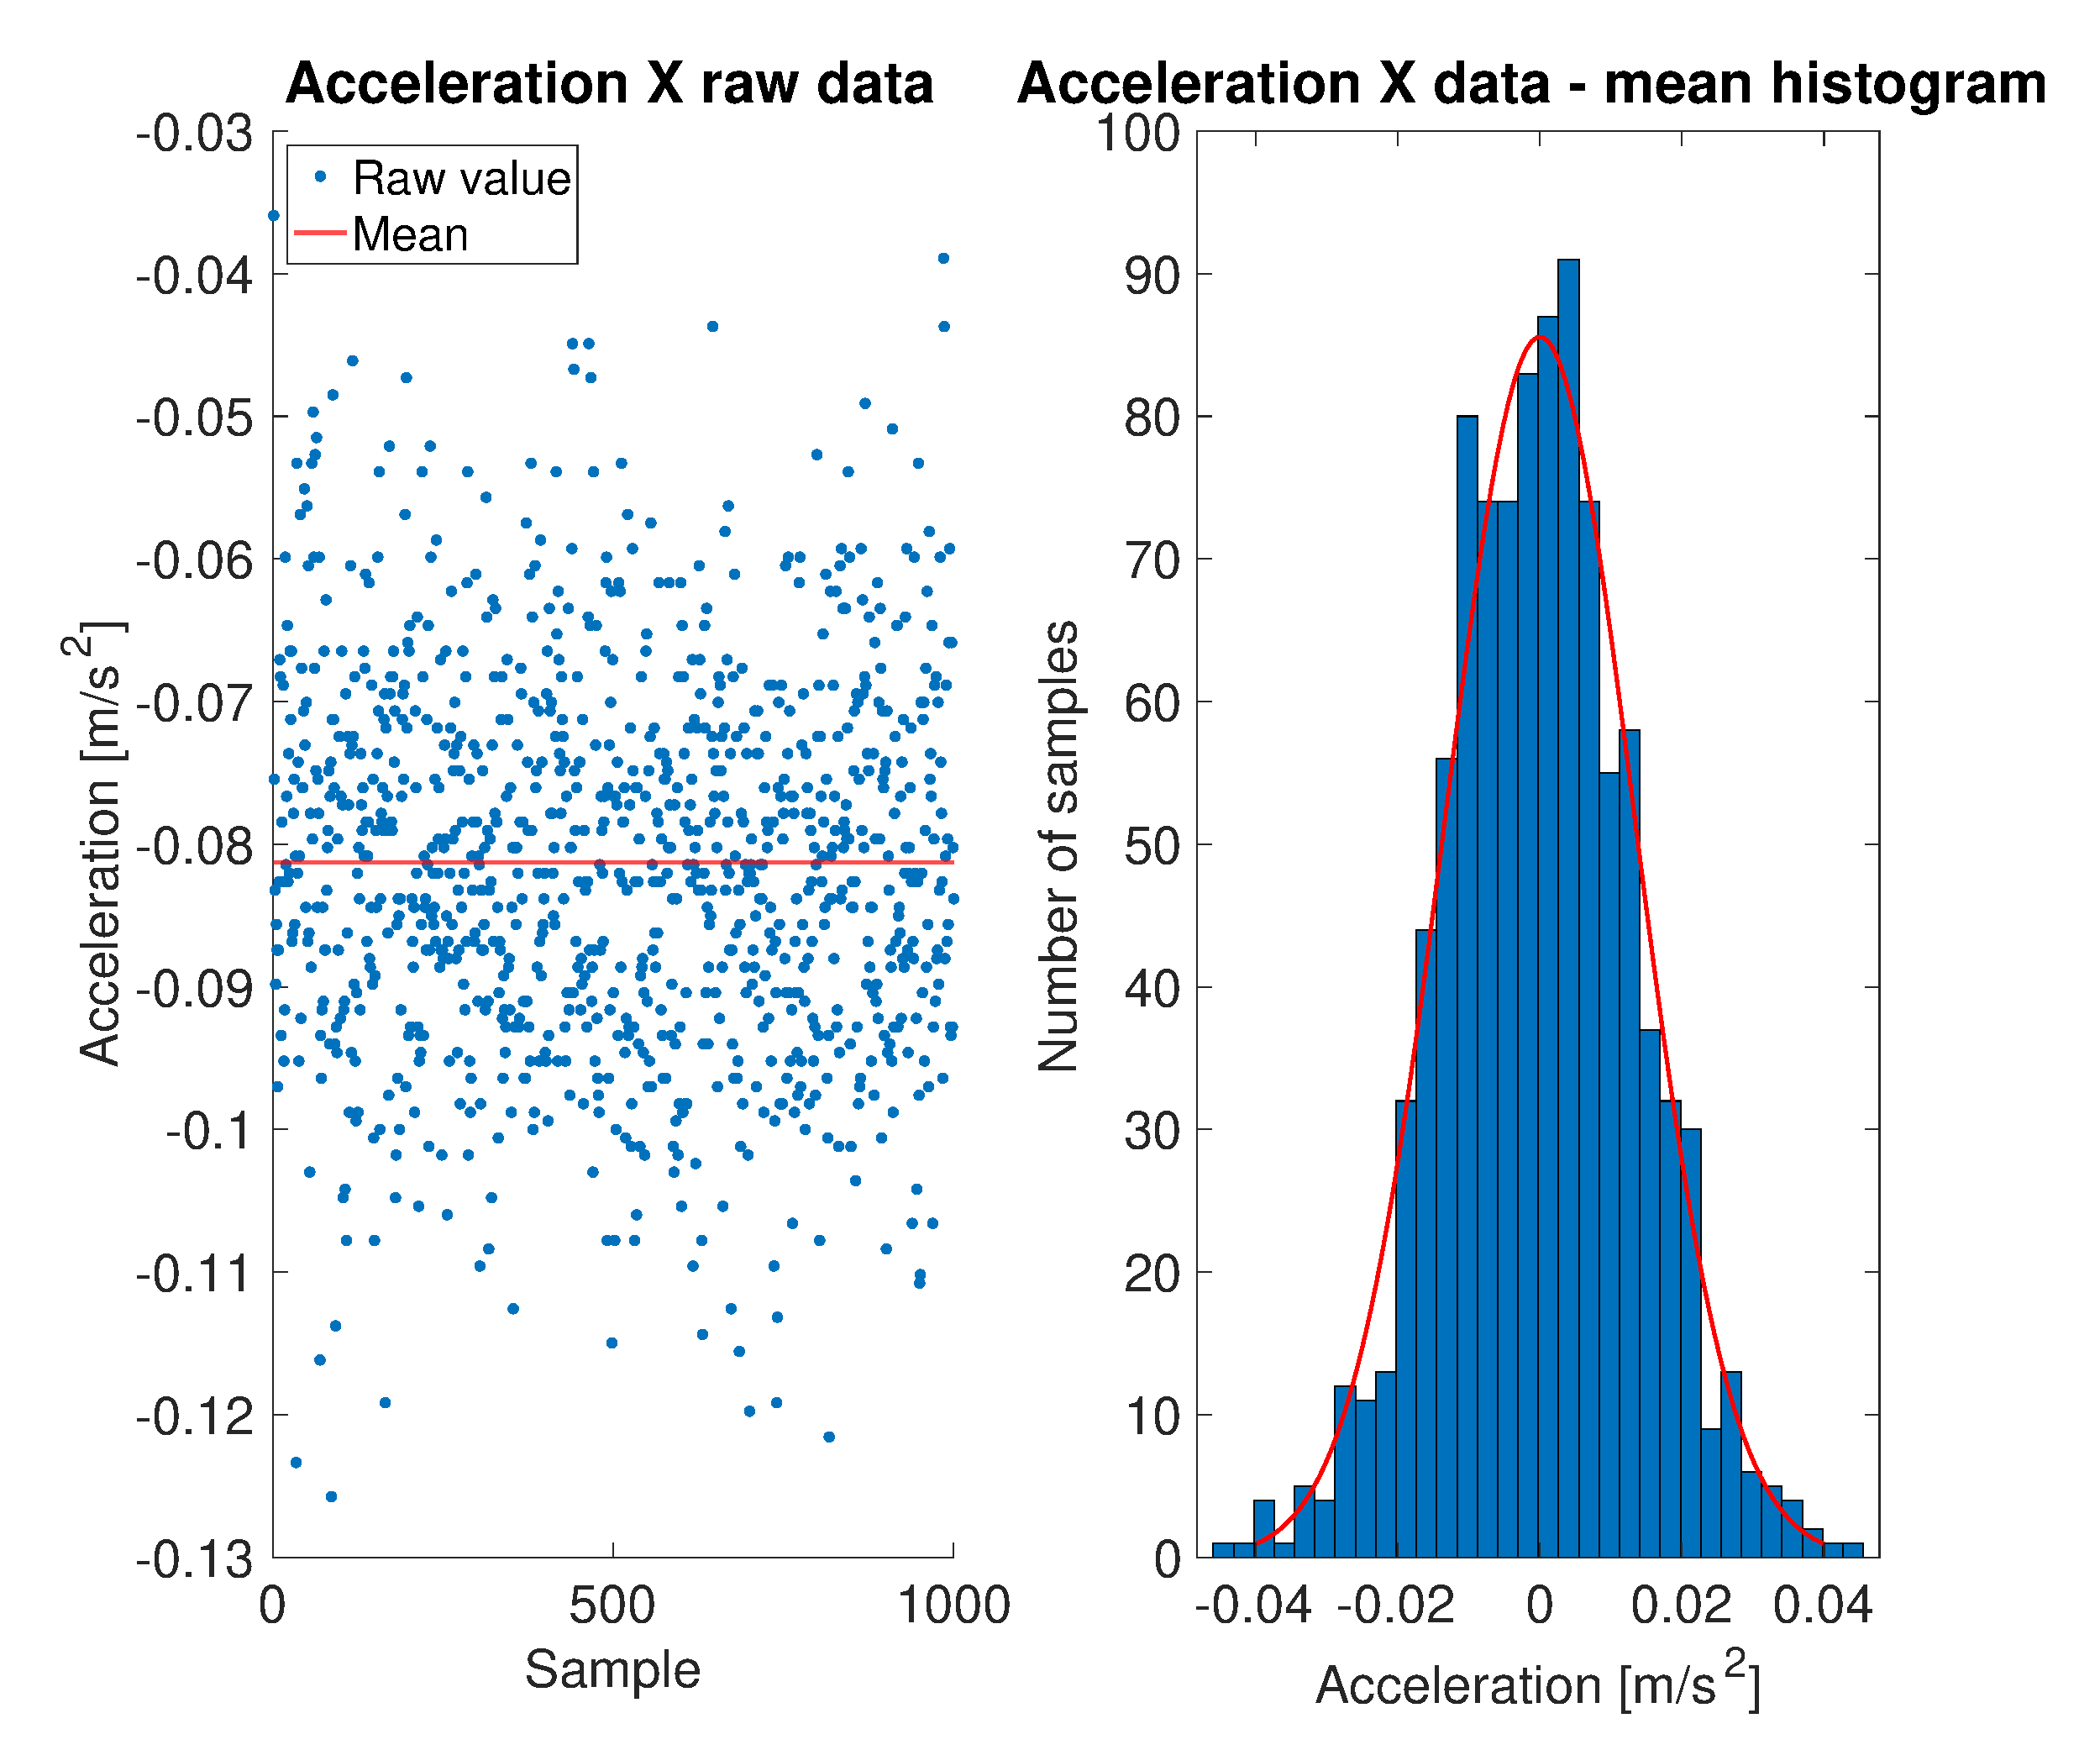
\includegraphics[width=.45\textwidth]{plots/plotAccelerationX}\hfill
        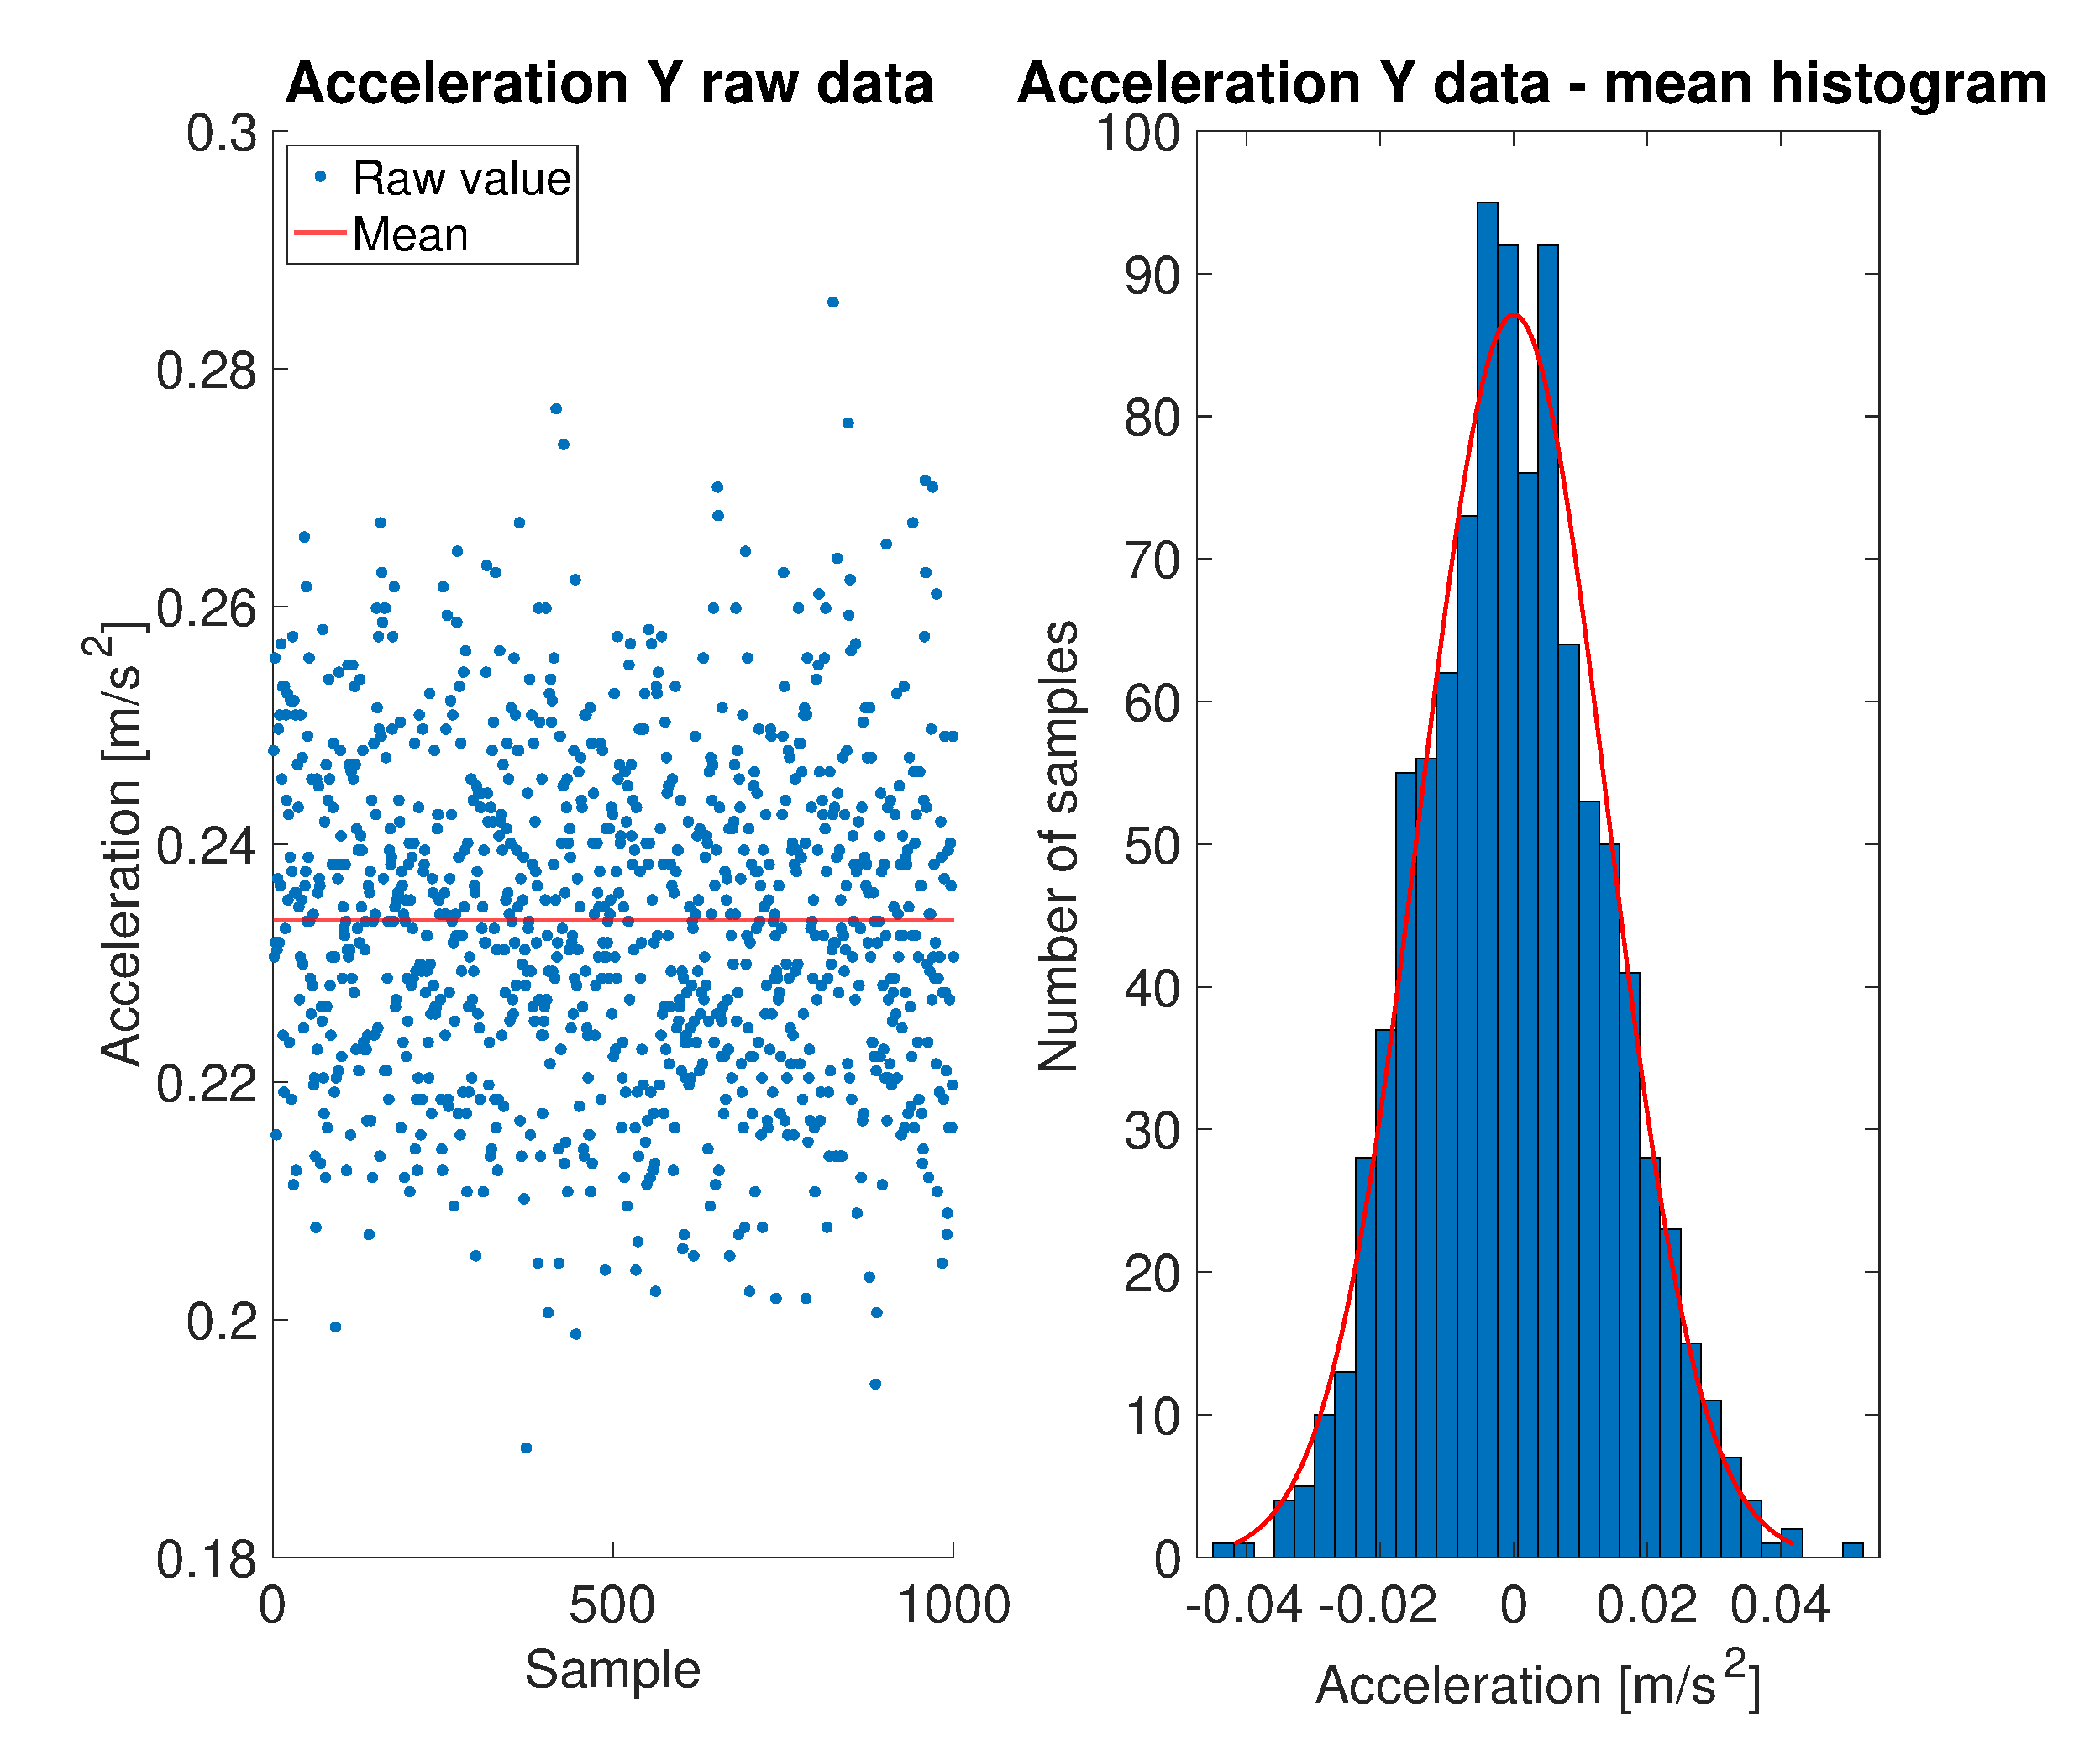
\includegraphics[width=.45\textwidth]{plots/plotAccelerationY}\vspace{1em}
        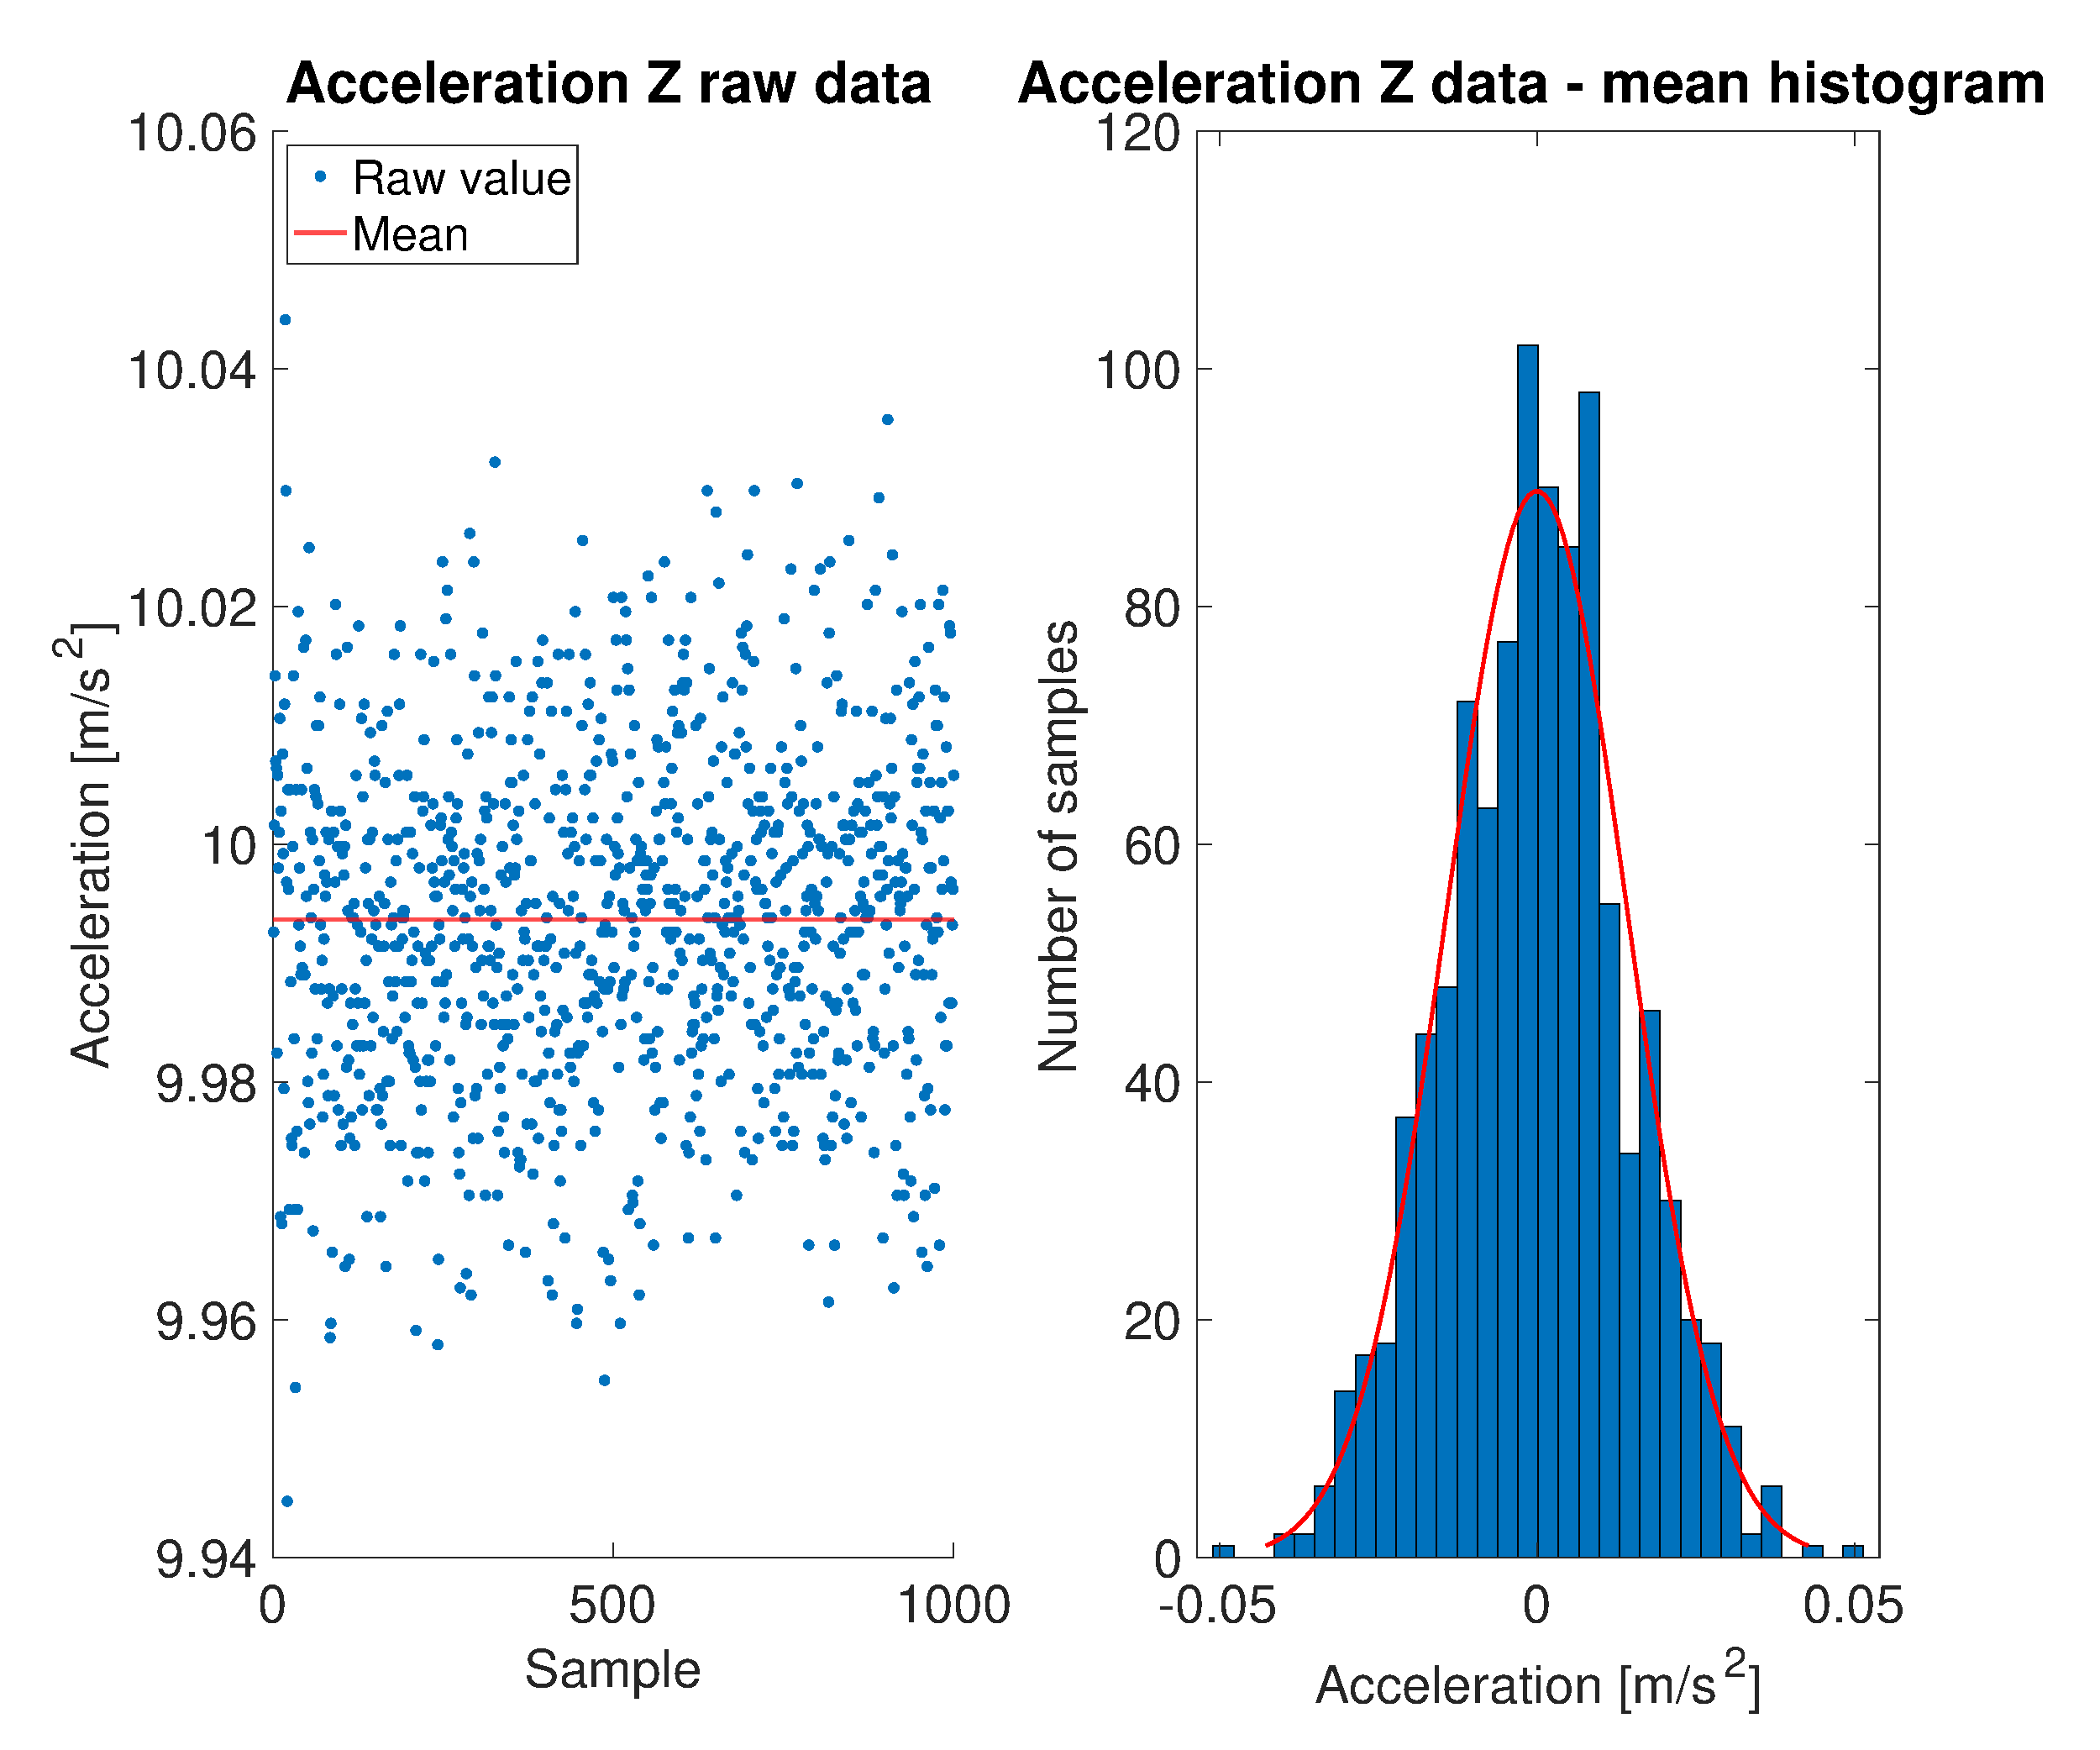
\includegraphics[width=.45\textwidth]{plots/plotAccelerationZ}\hfill
        \caption{Scatter raw data and histograms of the accelerometer reading at rest with subtracted offset. All three directions allow approximation by a normal distribution.}
        \label{fig:accelerationHist}
    \end{figure}

    \begin{table}[h]
        \begin{tabular}{lS[table-format=1.3]S[table-format=1.3]}
            \hline \vspace{-1em} \\
            Direction & {Mean value $\bar{\mathit{\Omega}}$ (offset) in \si{\degree\per\second}} & {Standard deviation $\sigma_\Omega$ in \si{\degree\per\second}} \\ \hline
            $x$       & -0.003                                                                   & 0.087                                                           \\
            $y$       & 0.009                                                                    & 0.102                                                           \\
            $z$       & 0.014                                                                    & 0.066                                                           \\ \hline
        \end{tabular}
        \caption{Summary of the rotation velocity $\mathit{\Omega}$ readings at rest, the number of samples was 1,000 in each direction. Please note the quantization of \SI{0.06}{\degree\per\second} for the individual values.}
        \label{tab:gyro}
    \end{table}
%    While the overall outcome was the same for the different repetitions, the starting phase strongly depended on
%    how the merry-go-round was pushed and differed for the different trials.
%    During the free ride, the rotational velocity decayed reproducibly, but it was sensitive to movements on
%    the merry-go-round, making this phase also prone to disturbances.
%
%    Figure~\ref{fig:gyro_decay} shows the rotational velocity of a typical ride (distance of the sensor from the
%    center was $r=\SI{0.7}{\metre}$).
%    After the maximum, the merry-go-round rode freely with decaying rotational velocity due to friction.
%    Without any external disturbances, the decay was linear.
%    A linear fit to the undisturbed phase led to a decay of the rotational velocity by \SI{0.8}{\degree\per\square\second}.
%    The coefficient of determination ($R^2$) for the fit was 0.98, confirming the assumption of a linear relationship
%    for the decay.

    \vspace{1em}

    \begin{figure}[h]
        \centering
        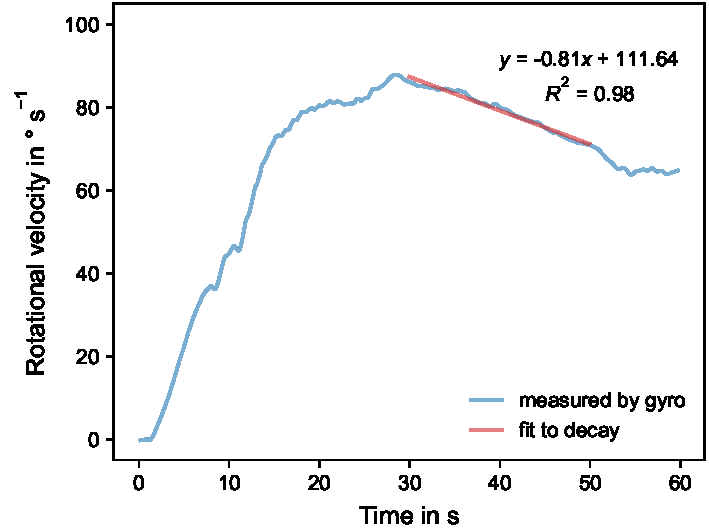
\includegraphics[width=.6\textwidth]{plots/gyro_2_decay.pdf}
        \caption{Rotational velocity measurement with a distance of the sensor from center $r=\SI{0.7}{\metre}$. The sensor values themselves were negative because of the clockwise rotation. Data were smoothed using a running average over 5 samples (\SI{0.5}{\second}).}
        \label{fig:gyro_decay}
    \end{figure}

%    \begin{table}[h]
%        \begin{tabular}{lS[table-format=1.3]S[table-format=1.3]}
%            \hline \vspace{-1em} \\
%            Direction & {Mean value $\bar{\mathit{\Omega}}$ (offset) in \si{\degree\per\second}} & {Standard deviation $\sigma_\Omega$ in \si{\degree\per\second}} \\ \hline
%            $x$       & -0.003                                                                   & 0.087                                                           \\
%            $y$       & 0.009                                                                    & 0.102                                                           \\
%            $z$       & 0.014                                                                    & 0.066                                                           \\ \hline
%        \end{tabular}
%        \caption{Summary of the rotation velocity $\mathit{\Omega}$ readings at rest, the number of samples was 1,000 in each direction. Please note the quantization of \SI{0.06}{\degree\per\second} for the individual values.}
%        \label{tab:gyro}
%    \end{table}
%    Evaluation of the data (Table~\ref{tab:gyro} shows summary of the mean values and corresponding standard deviations)
%    shows a very low offset (less than 1~LSB) and accordingly no significant difference between the directions.
%    Also the standard deviation below 2~LSB suggests a very low noise level.
%    The histograms (Figure~\ref{fig:gyro_hist}A--C) reveal the distribution more clearly.
%    Within the limits due to the quantization, the data allows approximation by a normal distribution.
%
%    The sensors for the rotation rate in $x$- and $y$-direction in the BHI260AP probably use a different setup than
%    for the $z$-direction, which could be based on out-of-plane motion.
%    However, even the histogram with the superimposed distributions (Figure~\ref{fig:gyro_hist}D)
%    shows no difference between the different axes.
%
%    \begin{figure}[h]
%        \centering
%        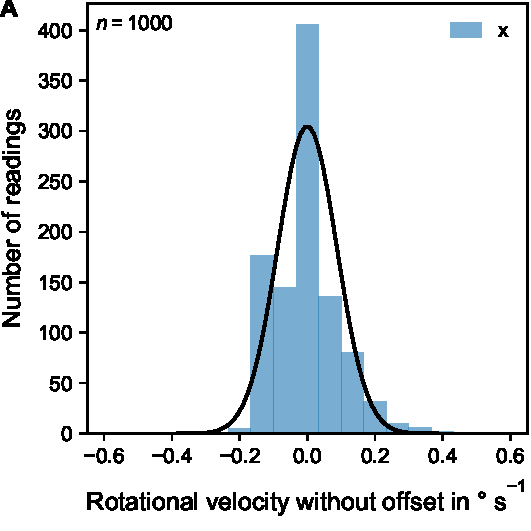
\includegraphics[width=.45\textwidth]{plots/gyro_hist_x.pdf}\hfill
%        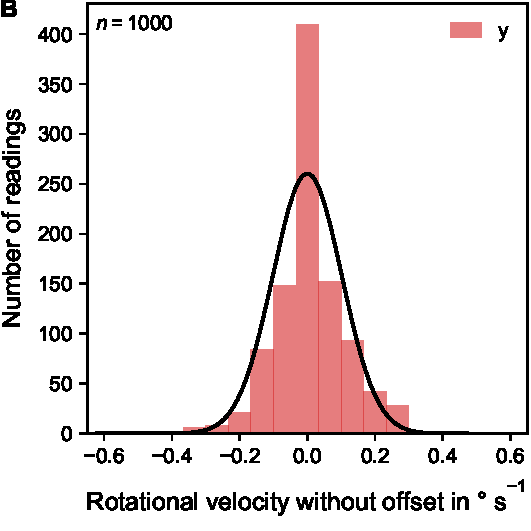
\includegraphics[width=.45\textwidth]{plots/gyro_hist_y.pdf}\vspace{1em}
%        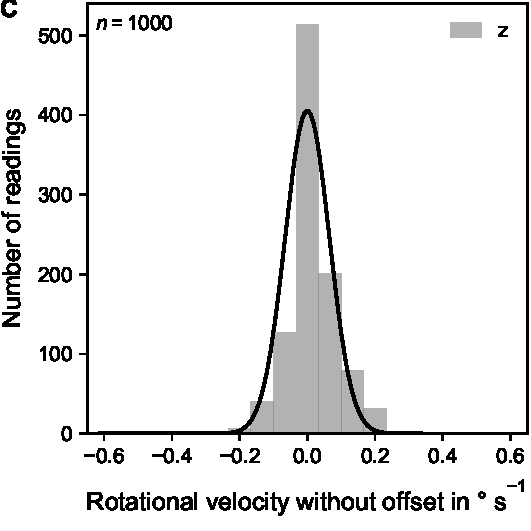
\includegraphics[width=.45\textwidth]{plots/gyro_hist_z.pdf}\hfill
%        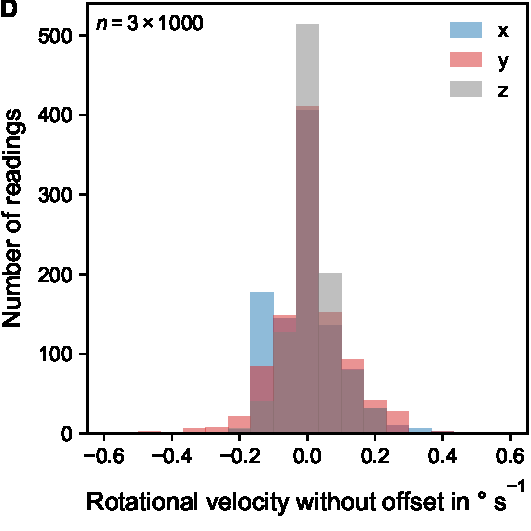
\includegraphics[width=.45\textwidth]{plots/gyro_hist_xyz.pdf}
%        \caption{Histograms of the gyroscope reading at rest with subtracted offset: all three directions allow approximation by a normal distribution (A--C), superposition of the three axis (D) show no clear difference between the directions.}
%        \label{fig:gyro_hist}
%    \end{figure}

    In parallel, the acceleration was measured (Figure~\ref{fig:acc}). The radial acceleration (positive sensor readings) followed the characteristics of the rotational velocity. In contrast, the signals appeared noisy, reflecting the vibrations of the merry-go-round. The tangential acceleration started with negative values during the up-ramping phase but reached positive values before the rotation maximum.

    However, the expected behavior would be that the tangential acceleration changes its sign only at the highest rotational rate, when the propelling of the merry-go-round ends. A possible explanation for this unexpected behavior is a slight misplacement of the Nicla Sense ME Board out of the exact radial axis. In this case, the much larger radial acceleration would superimpose and cause wrong tangential readings, especially for higher rotational velocities.

    \begin{figure}[h!]
        \centering
        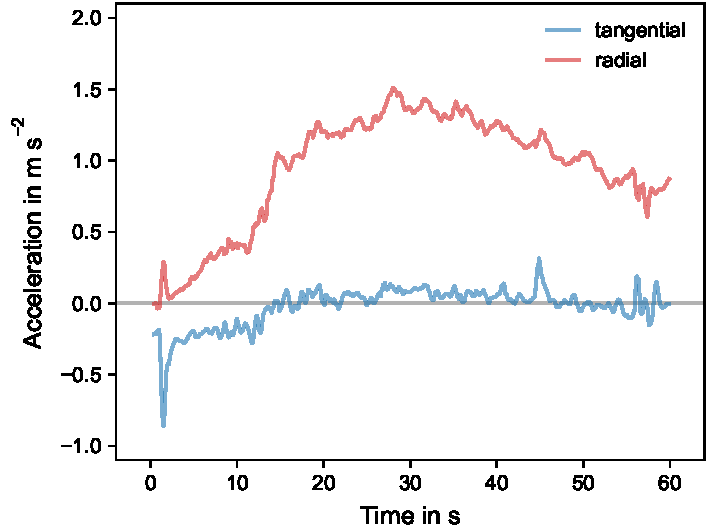
\includegraphics[width=.6\textwidth]{plots/acc_2.pdf}
        \caption{Acceleration measurement with a distance of the sensor from center $r=\SI{0.7}{\metre}$. The plot shows the run from Figure~\ref{fig:gyro_decay}. Data were smoothed using a running average over 5 samples (\SI{0.5}{\second}).}
        \label{fig:acc}
    \end{figure}

    Figure~\ref{fig:gyro_acc} shows the comparison between the rotational velocity measured by the gyroscope and the values calculated using the relationship of equation~2. For negative acceleration values at the beginning, no calculation was possible because of the square root. Especially for higher rotational speeds, the results match very well.

    \begin{figure}[h!]
        \centering
        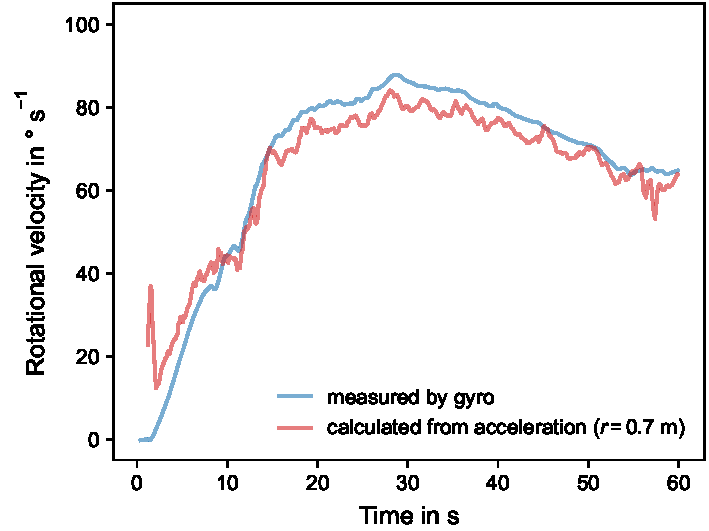
\includegraphics[width=.6\textwidth]{plots/gyro_2.pdf}
        \caption{Rotational velocities with a distance of the sensor from center $r=\SI{0.7}{\metre}$. The plot compares data measured by the gyroscope and values calculated from the radial acceleration. Data were smoothed using a running average over 5 samples (\SI{0.5}{\second}).}
        \label{fig:gyro_acc}
    \end{figure}

    \clearpage


    Table~\ref{tab:gyro_acc} summarizes the evaluation of the measured rotational velocity, the radial acceleration, and therewith calculated rotational velocity at the rotation maximum for the two different distances $r$ between the sensor and the center. Please note that the measured rotational velocity provides information about the direction (negative sign for clockwise rotation when the rotational velocity vector points upwards) in contrast to the value calculated from the radial acceleration. The discrepancy between the values is in both cases below \SI{10}{\percent}. Both, imprecision in $r$ as well as the fluctuations in the acceleration signal can contribute to this discrepancy.

    \vspace{2em}

    \begin{table}[h]
        \begin{tabular}{S[table-format=1.1]S[table-format=2.1]S[table-format=1.2]S[table-format=2.1]c}
            \hline \vspace{-1em}  \\
            {$r$ in \si{m}} & {$\mathit{\Omega}_\mathrm{z}$ in \si{\degree\per\second}} & {$a_\mathrm{y}$ in \si{\metre\per\square\second}} & {$\mathit{\Omega}_\mathrm{calc}$ in \si{\degree\per\second}} & Discrepancy \\ \hline
            0.7             & -87.9                                                     & 1.47                                              & 83.0                                                         & \SI{5.9}{\percent} \\
            1.0             & -83.1                                                     & 1.75                                              & 75.7                                                         & \SI{9.8}{\percent} \\ \hline
        \end{tabular}
        \caption{Comparison of the measured rotational velocity ($\mathit{\Omega}_\mathrm{z}$) to the calculated rotational velocity ($\mathit{\Omega}_\mathrm{calc}$) based on the radial acceleration ($a_\mathrm{y}$) for different distances $r$ between the sensor and the center. The discrepancy describes the relative deviation between the measured and calculated rotational velocity.}
        \label{tab:gyro_acc}
    \end{table}


    \section{Summary}
    Characterization of the gyroscope showed very low offset and noise, both in the range of the LSB. No differences between the three axes were observed. During merry-go-round rides, measurements with the gyroscope and the accelerometer provided realistic results for the rotational velocity, decay of the rotation due to friction, and radial acceleration. Calculating the rotational velocity from the centripetal acceleration lead to values matching well the results from the gyroscope.


% BibTeX or Biber would be better options, with just 2 reference the "raw" approach is fine for such a report
    \begin{thebibliography}{------}

        \bibitem[1]{labManual} J. Kieninger, S.\,J. Rupitsch, \textit{Sensors Lab Course}.
        University Freiburg.
        Winter term 2022/23.

        \bibitem[2]{BHI260} \textit{BHI260AP Datasheet}, Bosch Sensortec, BST-BHI260AP-DS000-02, rev. 1.1, 15-Apr-2021.
        \bibitem[3]{Hautala} Hautala, S., \textit{Physics Across Oceanography: Fluid Mechanics and Waves},
                             Available: https://uw.pressbooks.pub/ocean285/chapter/the-pgf/. [Accessed: 27-Nov-2022]

    \end{thebibliography}


\end{document}
